% This template is provided for all the participants of seminars
% offered by the database systems research group
% Adjusted for seminar "Information Networks"
%%%%%%%%%%%%%%%%%%%%%
% Author information:
%%%%%%%%%%%%%%%%%%%%%
% Jannik Strötgen
% Institute of Computer Science
% Database Systems Research Group
% INF 348 
% 69120 Heidelberg
% stroetgen@uni-hd.de
%%%%%%%
% Date: April 24, 2010
% minor modifications: October 17, 2011
% minor modifications: April 3, 2016 (Gertz)
% minor modifications: April 8, 2017 (Gertz)
% minor modifications: Dezember 4, 2018 (Gertz)
% minor modifications: April 5, 2020 (Gertz)
% minor modifications: April 1, 2021 (Gertz)
% minor modifications: February 18, 2022 (Gertz)
%%%%%%% 

\documentclass[
     11pt,         % font size
     a4paper,      % paper format
     oneside,
     ]{article}

%%%%%%%%%%%%%%%%%%%%%%%%%%%%%%%%%%%%%%%%%%%%%%%%%%%%%%%%%%%%

% PACKAGES:

% Use German :
\usepackage[USenglish]{babel}
% Input encoding
\usepackage[utf8]{inputenc}
% Font encoding
\usepackage[T1]{fontenc}
% Einbinden von URLs:
\usepackage{url}
% hyperrefs in the documents
\usepackage[bookmarks=true,colorlinks,pdfpagelabels,pdfstartview = FitH,bookmarksopen = true,bookmarksnumbered = true,linkcolor = black,plainpages = false,hypertexnames = false,citecolor = black,urlcolor=black]{hyperref} 
%\usepackage{hyperref}
% Include Graphic-files:
\usepackage{graphicx}
% Include PDF links
%\usepackage[pdftex, bookmarks=true]{hyperref}
% Fuer Textsatz
\usepackage{setspace}
\usepackage{parskip}
% For bibliography style
\usepackage[numbers]{natbib}
% for Latex symbols
\usepackage{doc}

\usepackage[ddmmyyyy]{datetime}
\usepackage{nth}
\usepackage{multirow}

\usepackage{amsfonts}
\usepackage{amsmath}
\usepackage{algorithm}
\usepackage{algorithmic}
\renewcommand{\algorithmicrequire}{\textbf{Input:}}
\renewcommand{\algorithmicensure}{\textbf{Output:}}

\usepackage{booktabs}
\usepackage{tabularx}
\usepackage{comment}


%%%%%%%%%%%%%%%%%%%%%%%%%%%%%%%%%%%%%%%%%%%
% Titel, Autor, Seminar, Semester, Dozent %
%%%%%%%%%%%%%%%%%%%%%%%%%%%%%%%%%%%%%%%%%%%
\newcommand{\mytitle}{Dense Retrieval with Entity Views}
\newcommand{\myauthor}{Johannes Gabriel Sindlinger}
\newcommand{\myseminar}{Modern Information Retrieval }
\newcommand{\mysemester}{Summer Term 2023}
\newcommand{\mydozent}{Prof.~Dr.~Michael Gertz}
\newcommand{\mydozentTwo}{Nicolas Reuter}
\newcommand{\mydozentThree}{Ashish Chouhan}
\newcommand{\mydozentFour}{Jayson Salazar}
\newcommand{\mydozentFive}{John Ziegler}
\newcommand{\myMatrikelnummer}{3729339}
\newcommand{\myStudiengang}{Master, Computer and Data Science}
\newcommand{\mySemester}{3}
\newcommand{\myEmail}{johannes.sindlinger@stud.uni-heidelberg.de}

% OTHER SETTINGS:
\setlength{\parindent}{0in}

% Pagestyle:
\pagestyle{myheadings}
\markright{\myauthor: \mytitle}

\begin{document}

%%%%%%%%%%%%%%%%%%%%%%%%%%%%%%%%%%%%% <TITLE> %%%%%%%%%%%%%%%%%%%%%%%%%%%%%%%%%%%%%
\pagenumbering{roman}
\begin{titlepage}
\begin{tabular}[l]{l}
% Angaben zum Seminar
Heidelberg University\\
Institute of Computer Science\\
\mysemester\\
Seminar: \myseminar\\
Instructors: \mydozent\\
\phantom{Instructors: }\mydozentTwo\\
\phantom{Instructors: }\mydozentThree\\
  \phantom{Instructors: }\mydozentFour\\
  \phantom{Instructors: }\mydozentFive
\end{tabular}

\vspace{4cm}
\begin{center}
\textbf{\large Seminar Paper} % Proseminararbeit,Studienarbeit, Interdisziplinaeres Projekt
\vspace{0.5\baselineskip}

% Titel wird ausgegeben (siehe oben)
{\huge
\mytitle
}
\end{center}

\vfill 
% Persönliche Angaben
\begin{tabular}[l]{ll}
Name:           & \myauthor\\
Student ID: & \myMatrikelnummer\\
Study Programme:    & \myStudiengang\ (\nth{\mySemester} semester)\\
Email: & \myEmail\\
Date of Submission: & \today \\
\end{tabular}

\end{titlepage}
%%%%%%%%%%%%%%%%%%%%%%%%%%%%%%%%%%%%% </TITLE> %%%%%%%%%%%%%%%%%%%%%%%%%%%%%%%%%%%%

% Zeilenabstand
\onehalfspacing


%%%%%%%%%%%%%%%%%%%%%%%%%%%%% <Antiplagiatserklärung> %%%%%%%%%%%%%%%%%%%%%%%%%%%%%
\thispagestyle{empty}
\vspace*{100pt}
I, \textbf{\myauthor}, hereby certify that I have written the paper entitled \textbf{\mytitle} in the seminar \textbf{\myseminar} in the \textbf{\mysemester} with \textbf{\mydozent} and \textbf{\mydozentTwo}, \textbf{\mydozentThree}, \textbf{\mydozentFour} and \textbf{\mydozentFive} independently and only with the aids indicated within the work.
I have clearly marked citations as well as the use of external sources, texts and aids according to the rules of scientific practice. \\

I am aware that I am not allowed to claim other people's texts and text passages as my own and that a violation of this basic rule of scientific work is considered an attempt to deceive and cheat, which will result in appropriate consequences. These consist of
the grading of the examination performance with \glqq not sufficient\grqq\ (5,0) as well as further measures if necessary. \\

Furthermore, I confirm that this work has not been presented in the same or similar form in any other seminar.
\vspace*{50pt}

Heidelberg, \today \hspace{2cm} \underline{\phantom{space for signature}}

\newpage
%%%%%%%%%%%%%%%%%%%%%%%%%%%%% </Antiplagiatserklärung> %%%%%%%%%%%%%%%%%%%%%%%%%%%%



%%%%%%%%%%%%%%%%%%%%%%%%%%%%%% <Inhaltsverzeichnis> %%%%%%%%%%%%%%%%%%%%%%%%%%%%%%%
% Table of contents
\tableofcontents
\newpage
%%%%%%%%%%%%%%%%%%%%%%%%%%%%%% </Inhaltsverzeichnis> %%%%%%%%%%%%%%%%%%%%%%%%%%%%%%





%%%%%%%%%%%%%%%%%%%%%%%%%%%%% <Hauptteil der Arbeit> %%%%%%%%%%%%%%%%%%%%%%%%%%%%%%
\pagenumbering{arabic}
\section{Introduction}\label{sec:introduction}

In the field of information retrieval, finding relevant information efficiently and effectively from large collections has been a challenge for a long time. This task involves finding documents or passages that are most relevant to a particular query or topic. Conventional methods of information retrieval often rely on sparse representations such as BM-25 (Robertson and Zaragoza \cite{BM25}), which can miss subtle semantic connections and fail to fully capture the context of the information being searched for.

Dense retrieval, on the other hand, has emerged as another approach that attempts to overcome the limitations of sparse representations by using dense vector embeddings of documents and queries. These embeddings are usually generated using large language models such as BERT (Devlin et. al \cite{bert}) and allow to encode richer semantic information. Consequently, they provide a more comprehensive understanding of the underlying content. 

For dense retrieval, two fundamentally different approaches have evolved: bi-encoder and cross-encoder. The bi-encoder approach involves creating distinct vector representations for queries and documents, which are then compared to determine relevance scores, while the cross-encoder approach directly measures the similarity between the query and document by taking both as input, potentially leading to more accurate results but with higher computational cost.

Apart from that, the field of information retrieval seems to evolve from a more classical approach of only ranking best matching documents of a related query to a 'rich search' (Balog \cite{balog2018entity}) ranking, which is often referred to 'Entity-oriented search', as Balog \cite{balog2018entity} describes. In this context, 'rich search' refers to the fact that answers to queries more often contain specific information about entities, facts or other structured data. In consequence, information about entities are quite relevant to solve this more sophisticated task.

However, large language models such as BERT tend to suffer from a problem that arises particularly in the context of querying documents: entities such as persons, locations, or organizations are not represented entirely within the models, as Heinzerling and Inui \cite{limitations} were able to illustrate. Thus, large language models are likely to represent socially relevant entities that occur in frequent documents, but at the same time entities that are rather rare not.

As an example, the two authors refer to the training process of BERT model, which uses a masked language model approach. During training phase, specific words or tokens are taken from existing documents and are randomly masked. The model is then charged to predict the masked tokens based on the context of the surrounding words. France is therefore correctly predicted with a high probability for the example 'Paris is the capital of [MASK]' (Heinzerling and Inui, \cite{limitations}), while prediction might be ambiguous for the rather rare entity Sesame Street in the case of 'Bert is a character on [MASK]' (Heinzerling and Inui, \cite{limitations}). In particular, entities that were not present during the training process and only emerged afterwards cannot be captured within language models at all.

The outlined relevance of entities in the retrieval of relevant information and the issue that these entities are not or only partially captured by large language models were the major reasons for Tran and Yates \cite{tran2022dense} to work on the paper that is presented in this seminar report. In the following, the work of Tran and Yates will be presented in detail and critically examined. The elaborations will be structured as follows: First, in \autoref{sec:related_work} the work is put into the context of current research in the field of information retrieval. Then, in \autoref{sec:methods}, the ideas and methods used by Tran and Yates are presented. This is followed by a presentation of the results in \autoref{sec:results}, before concluding with a critical assessment and personal opinion in \autoref{sec:discussion}.


\section{Related Work}\label{sec:related_work}

Entities have been a subject of interest in the field of information retrieval since the emergence of knowledge repositories like Wikipedia. Research in this context can be divided into the time before and after the advent of large language models such as BERT \cite{bert}.

\subsection{Entities in Sparse Retrieval}\label{subsec:sparse}

Prior to the advent of large language models such as BERT \cite{bert}, research focused on sparse retrieval methods like BM25, where entities from knowledge bases were used to enhance query understanding.  Efforts were made to expand queries using Wikipedia descriptions of entities \cite{xu2009query} and extract additional features like synonyms and relationships from linked knowledge bases \cite{dalton2014entity}. Balog \cite{balog2018entity} provided a comprehensive meta-analysis of related research.

\subsection{Entities in Dense Retrieval}\label{subsec:dense}

While some research has already addressed the consideration of entities in sparse retrieval, the amount of work in the field of dense retrieval in this context is rather limited. 

Some work focuses on integration of entities within interaction-based methods, treating textual and entity information as common inputs for ranking models. An example of this approach is the work of Xiong et al. \cite{xiong2017word,xiong2017word_2}: They developed a method to build ranking features by incorporating an attention mechanism of word embeddings and entity embeddings and could significantly outperform baselines for word-based and entity-based learning to rank systems.

Interaction-based methods such as these can be considered as extensions of the cross-encoder approach of dense retrieval and therefore potentially face the same issue of high computational complexity as described in \autoref{sec:introduction}. All documents and query pairs must be processed at runtime, which can lead to significant time and resource overhead. This leads to a slow overall retrieval process and can be inefficient, especially with large data sets.

In the context of the broad field of natural language processing tasks, entities have also been considered in several research papers and have been shown to have a significant impact on its tasks. The most prominent example is the ERNIE model (Sun et al. \cite{ernie}), which incorporates knowledge from both pre-training tasks and external knowledge graphs, enabling it to achieve better contextual understanding and knowledge integration in natural language processing tasks. 

ERNIE builds upon BERT's methods, particularly the masked language model, and tailors them to a more context-sensitive learning approach. ERNIE employs a masking strategy during its learning procedure, where the model is required to predict not only single words or tokens, but also several consecutive words. These consecutive words originate from different subtasks within the ERNIE model, including basic-level masking, phrase-level masking, and entity-level masking. The basic-level masking follows the standard token masking approach used in BERT, while the phrase-level masking groups small sets of tokens together to form conceptual units in the language to learn. Of most relevance to this seminar report is the entity-level masking stage, where the model tries to accurately predict entities that can span multiple tokens. This leads to the model becoming highly sensitive towards entities, as demonstrated by Sun et al. in their work on ERNIE \cite{ernie}. ERNIE can be fine-tuned for information retrieval tasks, offering valuable insights and serving as a reference model for Tran and Yates' work \cite{tran2022dense}.

The existing concepts of dense retrieval, including interaction-based methods and models like ERNIE, do not fully explore entities independently from the underlying large language model. This represents the main novelty of Tran and Yates' work \cite{tran2022dense}, which will be elaborated in the following sections.




\section{Methodology}\label{sec:methods}

As described above, the main contribution of Tran and Yates in the discussed work is to consider entities independently of the underlying large language model. In order to do so, they combine embeddings of an arbitrary large language model with embeddings of the entities from the respective documents and queries. For the embeddings of entities, they introduce some kind of multiple views on entities: Different sets of entities within queries and documents represent different perspectives on the queries and documents. Depending which view a query displays, different documents or parts of documents might be relevant.

In contrast to the previously described methods in \autoref{subsec:dense}, the separate embeddings of queries and documents are not inserted as components into a learned framework, but are merely merged into a joint vector space. As a result, a final embedding in the joint vector space is derived, which is used to calculate similarities between different vectors. Therefore, Tran and Yates, stick to the bi-encoder model (see \autoref{sec:introduction}), which allows indexing of embeddings for documents and enables fast ranking computations via ANN search. 

\subsection{General Model}\label{subsec:general_model}

The proposed method of Tran and Yates incorporates embeddings of documents and entities independently. To achieve a joined vector space, they merge embeddings of both for each query and document. This general approach is illustrated in \autoref{fig:general_model}: Since Tran and Yates follow the bi-encoder approach (see \autoref{sec:introduction}), embeddings for queries and documents are created independently of each other using a pre-trained large language model. 

\begin{figure}[!htb]
    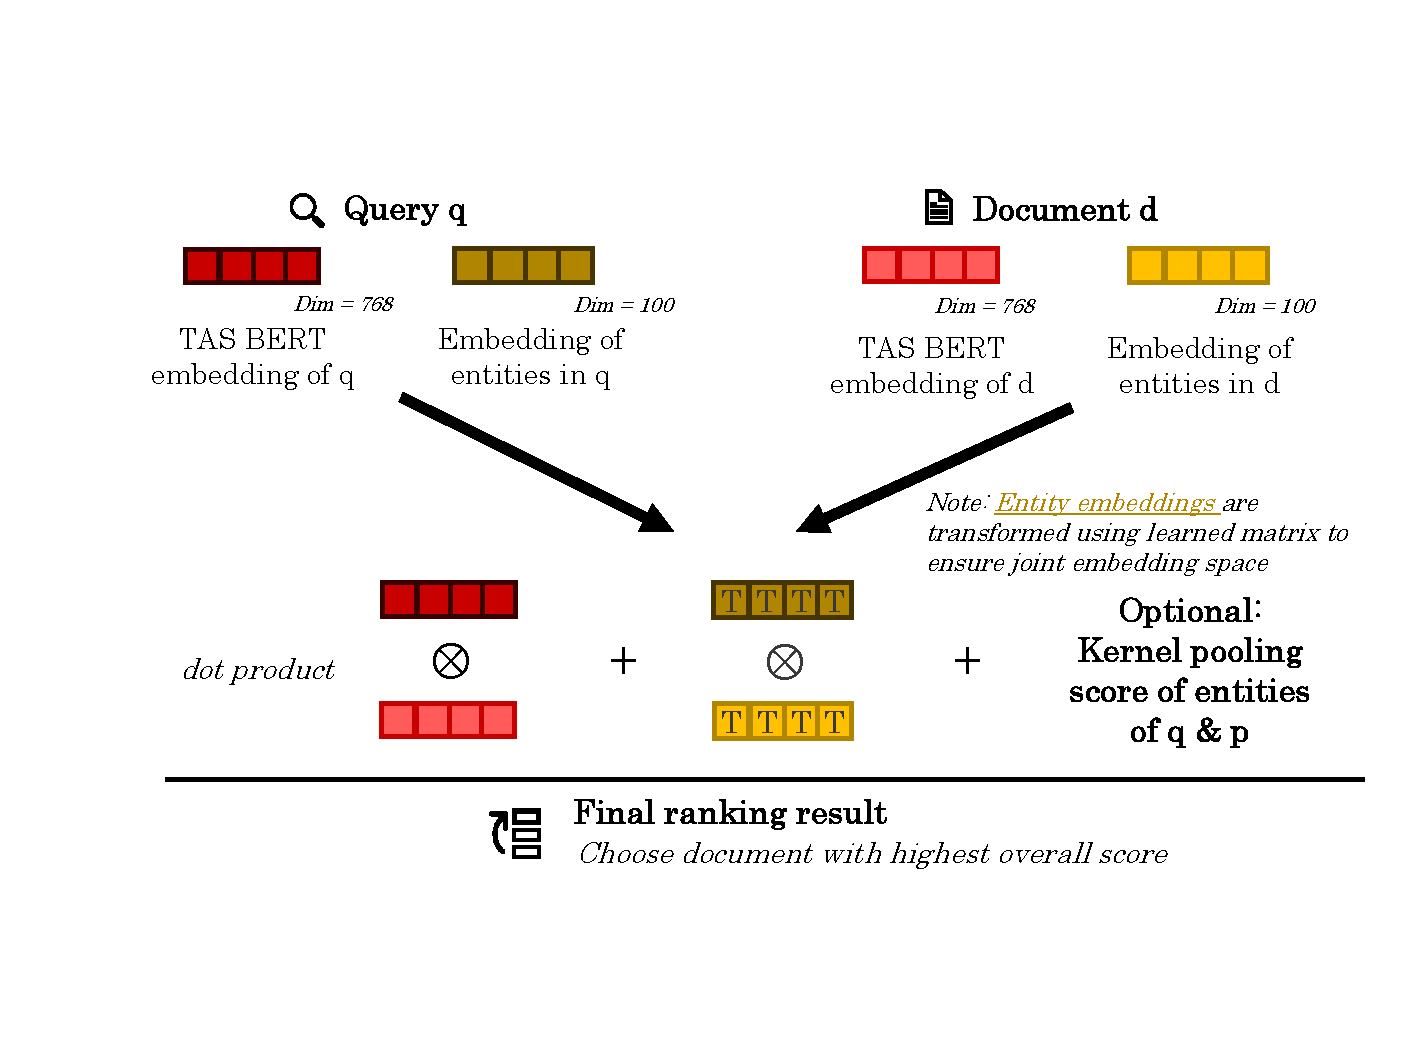
\includegraphics[trim={1.5cm 3cm 1.5cm 3cm}, clip, width=\textwidth]{resources/general_model} 
    \caption{General model}
    \label{fig:general_model}
\end{figure}

In their work, Tran and Yates use a distilled version of BERT (Sanh et al. \cite{sanh2019distilbert}), which was fine-tuned via TAS BERT approach by Hofst{\"a}tter et al. \cite{tasbert} for information retrieval task. The distilled version of BERT is used by Tran and Yates with the objective of maintaining low computational costs while losing little effectiveness. 

The term TAS BERT of the method of Hofst{\"a}tter et al. refers to the term 'topic aware sampled BERT', whereby sampling during training process of the information retrieval system is meant. In concrete, within TAS BERT approach the queries of the training dataset are clustered in advance based on different topics. During training process, query samples are extracted only from clusters of identical topics. This is intended to make the information retrieval model more sensitive to differing topics. 

In a usual dense retrieval setting, the generated embeddings of tokens are then compared using similarity measurements. When a query is submitted to a system, the ranking of the best documents with respect to the query is carried out, based on the calculated similarity score between the duets of the given query and all documents. 

For their model, Tran and Yates use the identical principle, but enhance it with embeddings of entities. In addition to the textual embeddings of a pre-trained language model, for each query and each document a single entity embedding is generated. Subsequently, the textual embedding is combined with the entity embedding in order to create an embedding that contains both the information about the semantic context and the information about the entities. The term combination here refers to concatenation of both vectors. 

Experimental results of Tran and Yates showed that concatenation yields the best results for combining both embeddings of text and entities compared to others like max pooling and sum pooling. \autoref{tab:operator} displays the respective analysis of Tran and Yates based on their experimental setup, which is introduced in detail in \autoref{sec:results}. Apart from the analytical point of view, the approach of concatenation offers the advantage that it can be understood quite intuitively.

\begin{table}[!htb]
    \centering
    \begin{tabular}{llll}
    \hline
    \multirow{2}{*}{\textbf{Operators}} & \multicolumn{3}{c}{\textbf{MS MARCO Dev}}   \\
                                      & \textbf{nDCG} & \textbf{MRR} & \textbf{MAP} \\
    \hline
    Sum & 0.393 & 0.335 & 0.339 \\
    Max & 0.388 & 0.330 & 0.334 \\
    Concat & 0.396 & 0.341 & 0.343 \\
    \hline
    \end{tabular}
    \caption{Varying Aggregation Operators of Embedding Concatenation}
    \label{tab:operator}
\end{table}

However, there is an issue to be solved in the context of concatenation: Since the vectors of the word embeddings and the entity embeddings are generated in a different vector space, this setup leads to biased similarity results. More precisely, the dimension of the word embeddings of the distilled TAS BERT model is 768 and of the word embeddings 100. Moreover, the magnitudes of the embeddings do not necessarily coincide. To overcome this problem, Tran and Yates introduce a transformation matrix $W \in \mathbb{R}^{100 \times 100}$ for the vectors of the embeddings. So let $\mathbf{E}(t)$ be the embedding of entities of text $t$, the transformed entity embedding is given as:
\begin{align}
    \mathbf{R}_{entity}(t) = W^T \cdot \mathbf{E}(t)
\end{align}
The values of the matrix are determined during the training process of the entire model and thus reflect a meaningful transformation of the embeddings into a joint vector space. 

Given text $t$ and its corresponding word embedding $\mathbf{R}_{text}(t)$ derived by the pre-trained language model, the final vector representation of $t$ is then calculated as:
\begin{align}
    \mathbf{R}_{final}(t) &= \mathbf{R}_{text}(t) \oplus \mathbf{R}_{entity}(t)
\end{align}

As a further optional addition to their model, Tran and Yates include an external scoring source that measures the relationship between query entities and documents. They use a kernel pooling score that is intended to measure the importance of entities of queries which also occur within documents. Accordingly, this approach requires knowledge of the query and document at runtime. Therefore, this approach belongs to methods interaction-based approaches of incorporating entities within retrieval tasks, as described in \autoref{sec:related_work}.

This kernel pooling score, called KNRM-signal will be elaborated in detail in the following subsection. Together with the KNRM-signal $S_{knrm}$ of a query $q$ and a document $d$ the final vector representation of the model of Tran and Yates resolves to 
\begin{align}
    \mathbf{R}_{final\_knrm}(t) =
    \begin{cases}
         \mathbf{R}_{text}(t) \oplus \mathbf{R}_{entity}(t) + 1 & t \text{~is query} \\
         \mathbf{R}_{text}(t) \oplus \mathbf{R}_{entity}(t) + S_{knrm}(t) & t \text{~is document} \label{eq:knrm}
    \end{cases}
\end{align}

Since the interaction of entities in queries with each other is always ideal, the maximum value $S_{knrm}(t)$ will be reached whenever $t$ is a query. As shown in \autoref{subsec:knrm}, the supremum of $S_{knrm}(t)$ is 1, therefore the value for $S_{knrm}(t)$ is set to 1, if t is a query.

\subsection{KNRM Signal}\label{subsec:knrm}

Tran and Yates introduce the KNRM signal, originally developed by Xiong et al. \cite{xiong2017end}, as an additional scoring mechanism to extend their basic approach by a separate framework. Unlike its original use, Tran and Yates adapt the KNRM model to specifically capture the interaction between entities in queries and documents. The calculation of the KNRM signal follows these steps:

\begin{enumerate}
    \item Let $X(q)$ be the set of all entity embeddings within query $q$, $X(d)$ any set of entity embeddings which occur in document $d$. For EVA Single and EVA Single-QA models (see \autoref{subsec:models}) $X(d)$ contains all entities with the given document, for EVA Multi (see \autoref{subsec:models}) $X(d)$ contains only entities of specific subsets of entities of $d$. The entity interaction matrix is defined as: 
    \[T_{i,j} := sim(X_i(q), X_j(d)) \text{~,}\]
    where $X_i(q)$ and $X_j(d)$ are the $i$-th and $j$-th embedding of $q$ and $d$. The similarity function is given as cosine similarity. Embeddings are generated via Wikipedia2Vec (Yamada et. al \cite{yamada2018wikipedia2vec}), as described in \autoref{subsubsec:extracting_entities}.
    \item Build k kernels using radial basis function, which creates differentiable histograms around given $\mu$ and $\sigma^2$.
    \[ K_l(X_i(q)) = \sum_{j=1}^{|X(p)|}\exp\left(-\frac{(T_{i,j}-\mu_i)^2}{2\sigma_i^2}\right)\]
    \item Pool / Summarize the k results into a k-dimensional feature vector: \[\overrightarrow{K(X_i(q))} = [K_1(X_i(q)), \ldots, K_k(X_i(q))]\]
    \item Build kernel-pooled representation $\phi(T)$ by calculating log-sum for each query entity: \[\phi(T) = \sum_{i=1}^{|X(q)|} \log \overrightarrow{K(X_i(q))}\]
    \item Get final kernel pooling score by applying a learned ranking layer. Note that $\tanh(\cdot) \in (-1, 1)$ and therefore $\sup S_{knrm} = 1$: \[ S_{\text{knrm}} = \tanh(w^T\phi(T) + b) \]
  \end{enumerate}

Despite being an interaction-based model that requires scoring during runtime for all query-document pairs, the computational complexity of the KNRM approach remains limited. The computations involved are relatively straightforward, and the additional learned layer does not significantly increase the computational overhead. Furthermore, these computations can be performed in parallel with the other components of Tran and Yates' approach. Empirical results concerning the latency of the models, with and without the KNRM signal, validate this assertion (see \autoref{sec:results}).

\subsection{Generating Entity Embeddings\label{subsec:entity_embeddings}}

As described in \autoref{subsec:general_model}, Tran and Yates create embeddings for both word tokens and entities in queries and documents. While the word token embeddings are generated using TAS BERT through the dense retrieval approach, the primary focus of their contribution lies in the creation of entity embeddings. In particular, since queries and documents usually contain more than one entity, they need to be aggregated to a single embedding.

In order to do so, the example given in \autoref{fig:example} shall be introduced: Given the query 'Favourite book bert sesame street' and a corresponding document that mentions Bert as a character of Sesame Street who enjoys the book Boring Stories, there are three entities: Bert, Sesame Street, and Boring Stories.

\begin{figure}[!htb]
    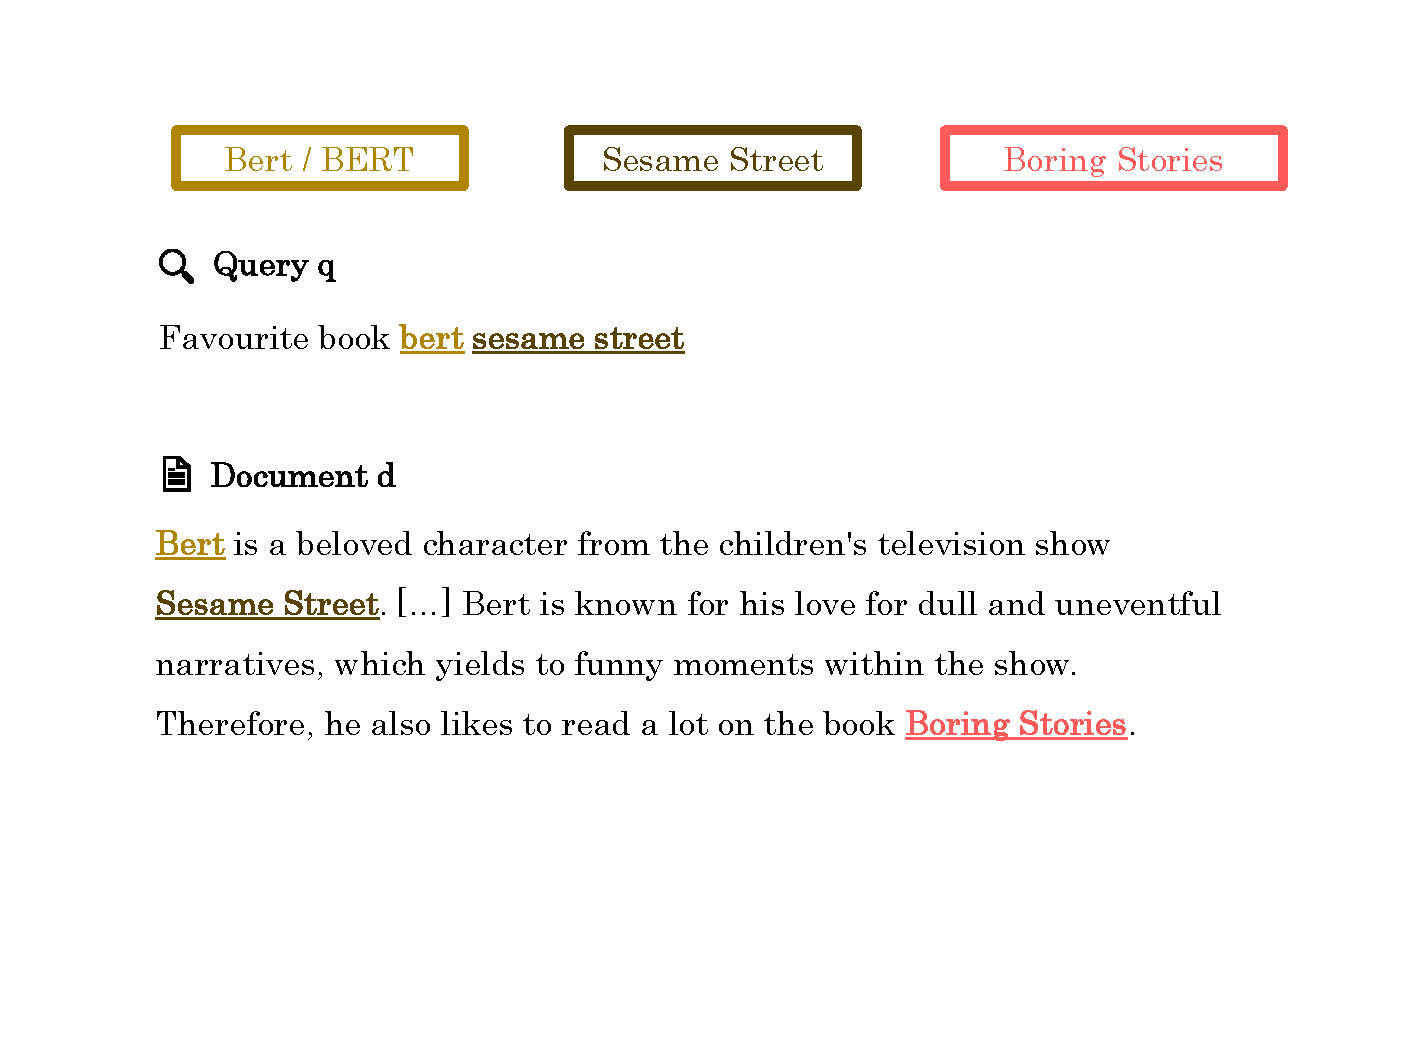
\includegraphics[trim={1.5cm 5.5cm 1.5cm 2cm}, clip, width=\textwidth]{resources/example} 
    \caption{Example query and example document}
    \label{fig:example}
\end{figure}

\subsubsection{Extracting Entities}\label{subsubsec:extracting_entities}

To aggregate multiple entities in a document or query, Tran and Yates first extract these entities from the text using external frameworks Dexter (Ceccarelli et al. \cite{ceccarelli2013dexter}) and Wikipedia2Vec (Yamada et. al \cite{yamada2018wikipedia2vec}).

The Dexter framework is an entity linkage system that resolves entity mentions in text to corresponding entities in a knowledge base. In particular, Dexter employs a combination of methods, including named entity recognition and pattern matching, to perform this task. 

Wikipedia2Vec, on the other hand, leverages the structure of Wikipedia to generate dense vector representations (embeddings) for words, articles, and entities. It utilizes the Word2Vec algorithm (Mikolov et al. \cite{mikolov2013distributed}) to capture semantic relationships from Wikipedia, producing high-dimensional embeddings.

The extraction procedure involves submitting a document or query to Dexter, which extracts entity mentions from the given text. These entity names are then passed on to the knowledge base, which transforms them into embeddings. Wikipedia2Vec provides vectors in dimension 100 as default, Tran and Yates keep this value in their model. \autoref{fig:entity_extraction} visualizes this process.

\begin{figure}[!htb]
    \centering
    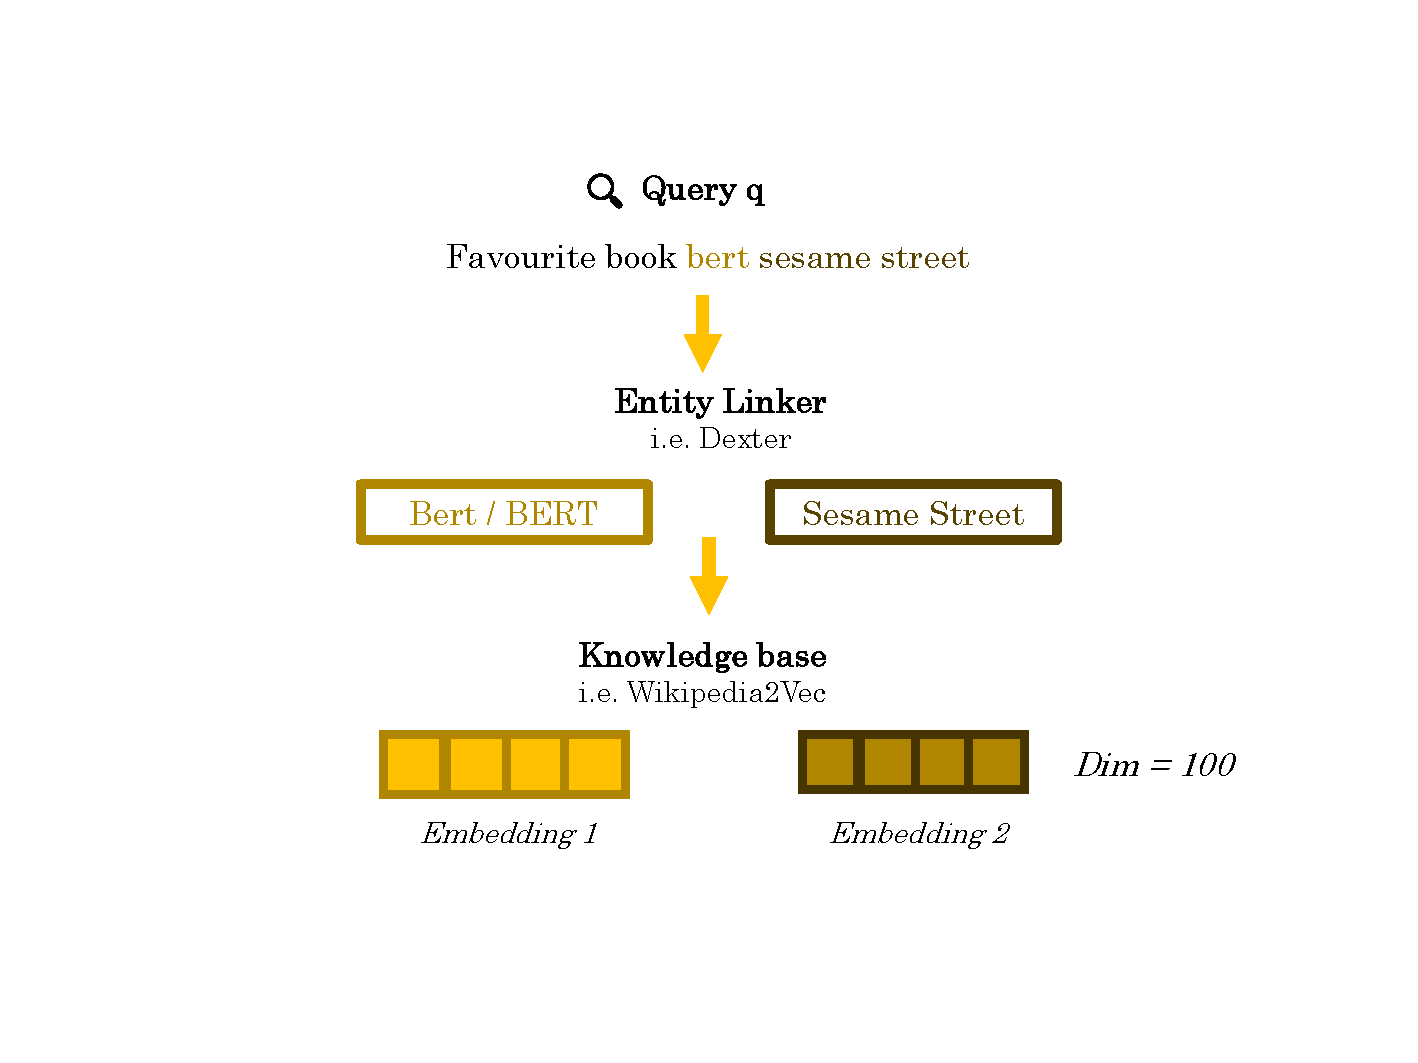
\includegraphics[trim={2cm 3cm 2cm 2cm}, clip, width=0.9\textwidth]{resources/entity_extraction} 
    \caption{Process of entity extraction}
    \label{fig:entity_extraction}
\end{figure}

\subsubsection{Combining Entities for Queries}\label{subsub:generating_queries}

For now, multiple embeddings for each entity within a query or a document are generated by applying the procedure outlined in \autoref{subsubsec:extracting_entities}. The aggregation of these generated embeddings differs based on whether a query or a document is considered, given the usual brevity of queries compared to documents.

For queries, Tran and Yates adopt a straightforward approach. They aggregate the embeddings of entities by averaging all entity embeddings across all dimensions. \autoref{fig:queries} visualizes this procedure.

\begin{figure}[!htb]
    \centering
    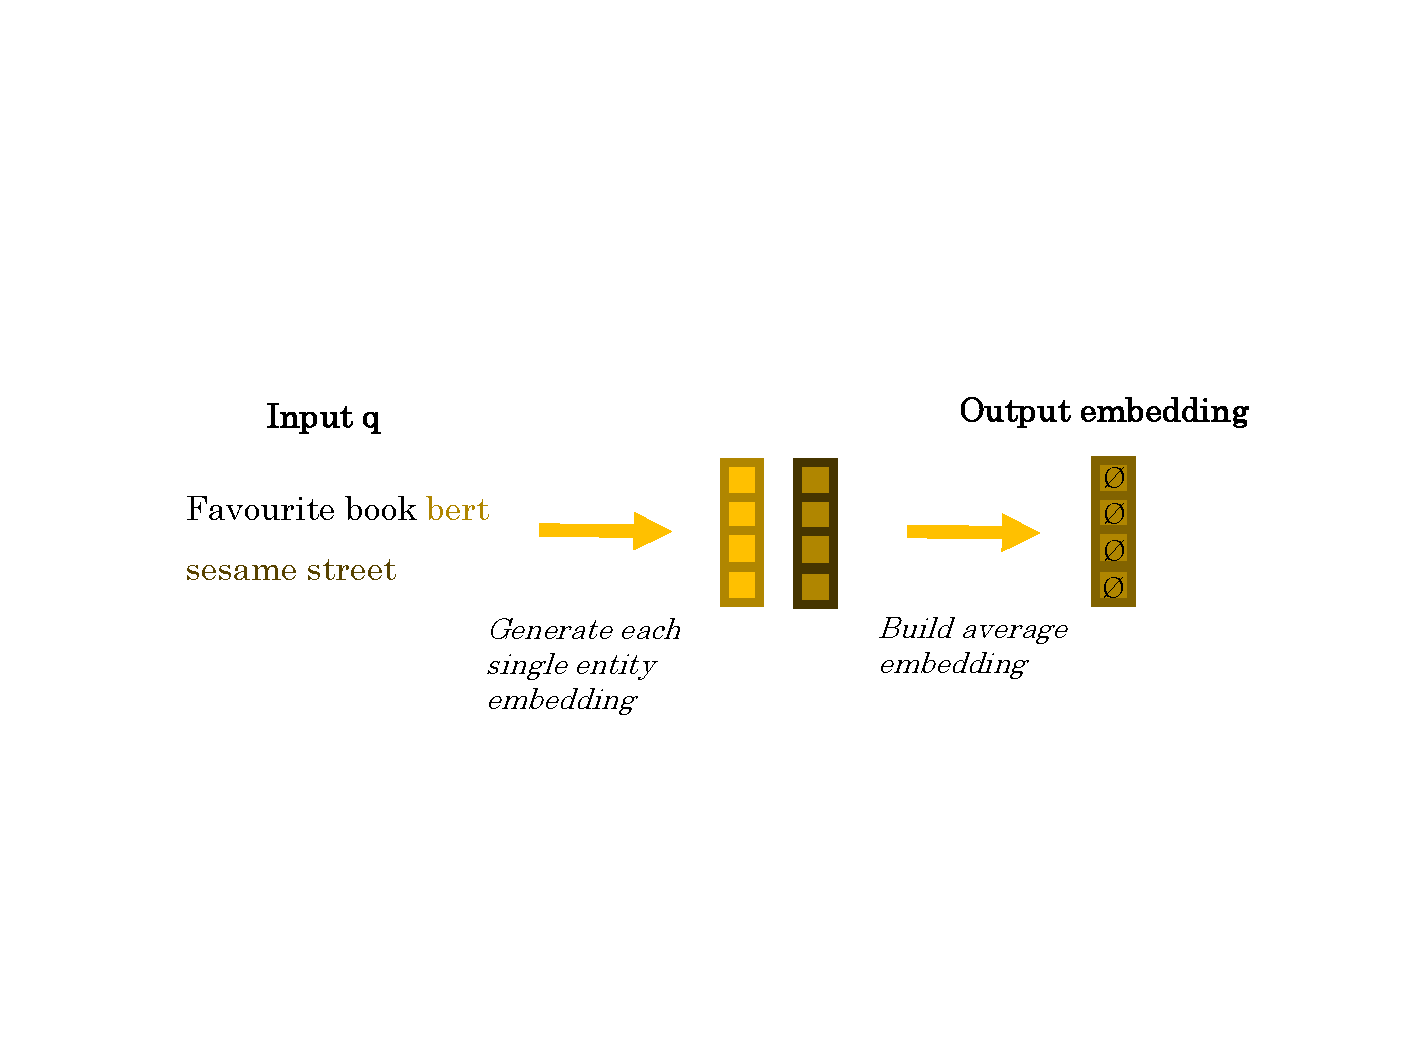
\includegraphics[trim={2cm 6cm 2cm 6cm}, clip, width=\textwidth]{resources/queries} 
    \caption{Process of generating a single entity embedding for a query}
    \label{fig:queries}
\end{figure}

\subsubsection{Combining Entities for Documents}\label{subsec:models}

Documents usually contain many different entities, as the example in \autoref{fig:example} indicates. Additionally, documents might also cover different aspects of a topic, so entities from very different areas might appear within them. This factor adds more complexity to the aggregation of embeddings for documents than for queries. To overcome this issue, Tran and Yates elaborated three different methods to aggregate embeddings of documents, which build upon each other:

\begin{itemize}
    \item Single Entity Representation (EVA Single)
    \item Query-Aware Single Entity Representation (EVA Single-QA)
    \item Multiple Entity View Representation (EVA Multi)
  \end{itemize}

The term EVA refers to \underline{E}ntity \underline{V}iews in Dense Retriev\underline{a}l. The concept of Entity Views, the name-giving term for the paper by Tran and Yates, is used in particular in the third method EVA Multi and will be introduced in the following.

\paragraph*{EVA Single}

The first approach of aggregating the entities of a document is similar to the one used for queries. The idea of the Single Entity Representation approach is to extract all entities of a document and then create a single average output embedding. Analogous to \autoref{fig:queries} for queries, this approach is visualized in \autoref{fig:eva_single}.

\begin{figure}[!htb]
    \centering
    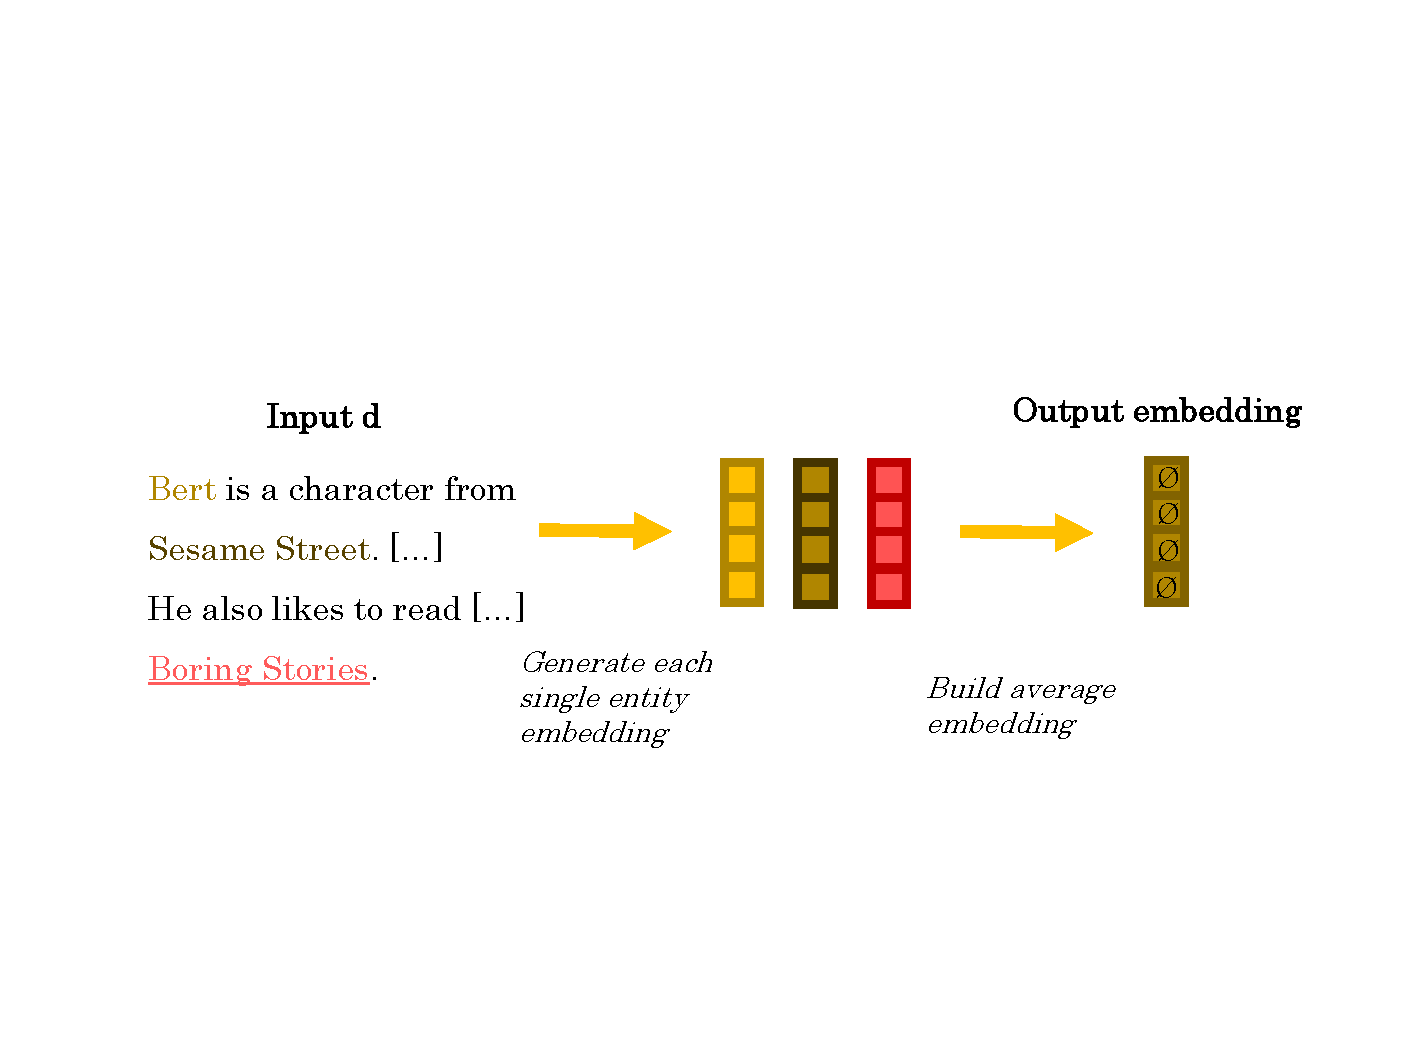
\includegraphics[trim={2cm 6cm 1.5cm 6cm}, clip, width=\textwidth]{resources/eva_single} 
    \caption{Process of generating an entity embedding for a document following the EVA Single approach}
    \label{fig:eva_single}
\end{figure}

This approach does not take into account that documents can cover various topics. The query information is completely discarded and thus partially irrelevant entities are accounted for calculations of the output embedding. This leads to a bias within the ranking results, as it can be observed in \autoref{sec:results}.

\paragraph*{EVA Single-QA}

To address this problem, Tran and Yates introduce the Query-Aware Single Entity Representation, which creates embeddings focusing on the needs of the query. However, this requires the assumption that the query is known before calculations, which leads to increased computational complexity. This is due to the fact that computations for all duets of query and documents must now be performed during runtime, precomputations of embeddings for documents and indexing is no longer possible. This effect is reflected within the results (see \autoref{sec:results}), which prove a high latency in the case of the EVA-Single QA approach.

The underlying idea of the EVA single QA model is to filter the entities of a document based on the information of a given query and select only entities with high similarity to a query entity. \autoref{fig:eva_single_qa} visualizes this process.

\begin{figure}[!htb]
    \centering
    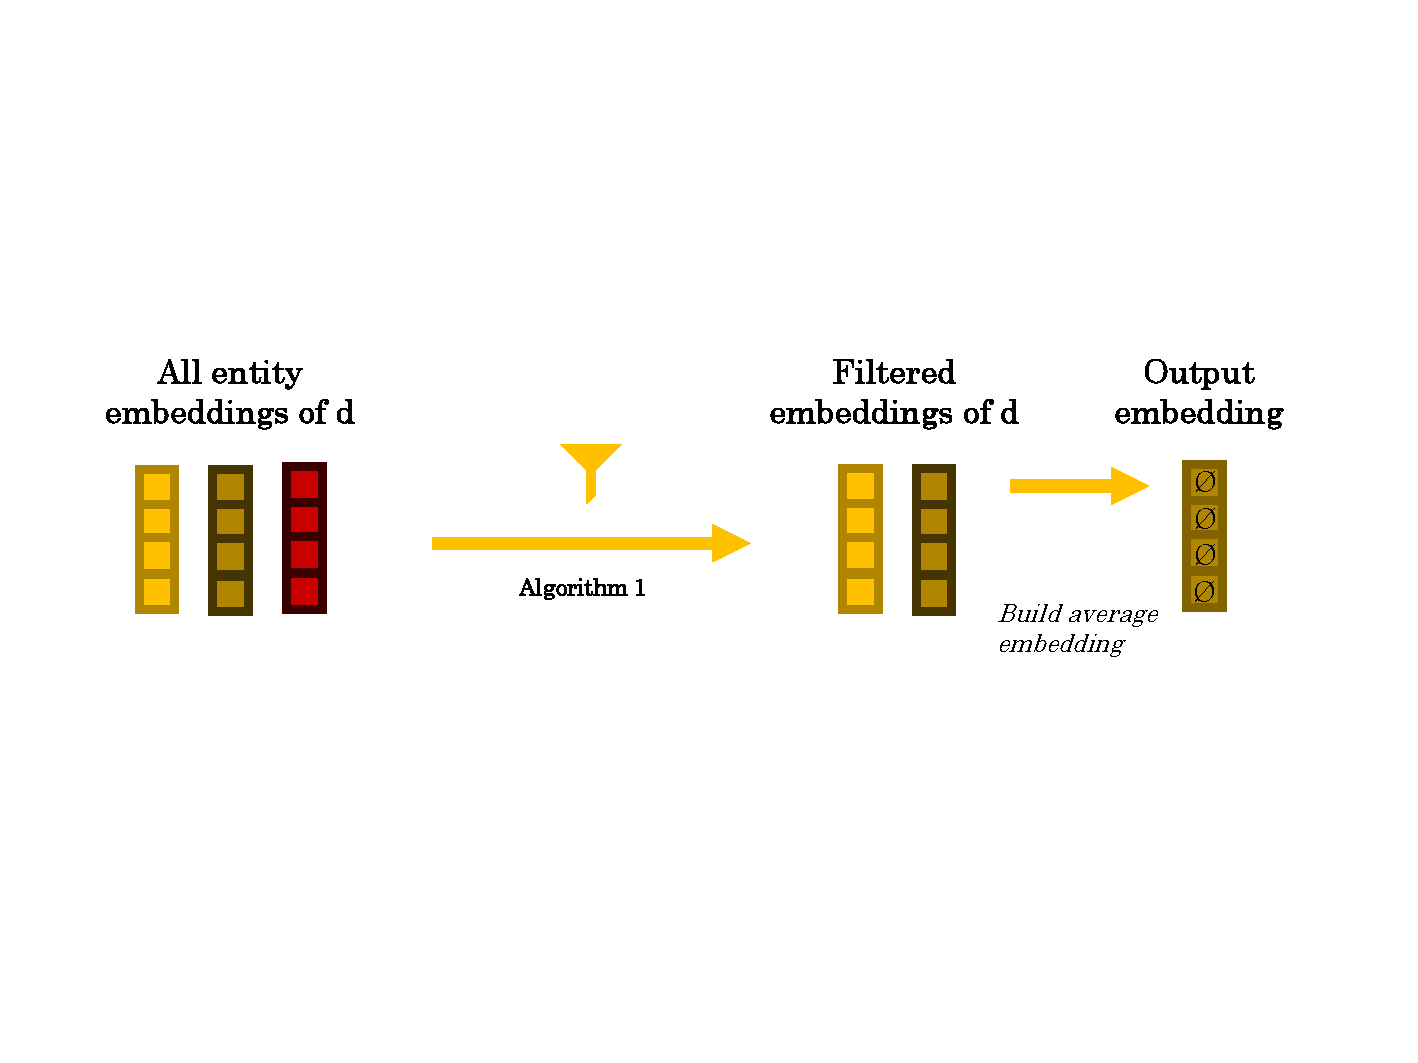
\includegraphics[trim={1cm 6.5cm 2cm 6cm}, clip, width=\textwidth]{resources/eva_single_qa} 
    \caption{Process of generating an entity embedding for a document following the EVA Single-QA approach}
    \label{fig:eva_single_qa}
\end{figure}

Filtering is done using algorithm \ref{alg:query-aware-entity-representation}, which is applied to all duets of a query $q$ and document $d$: For each entity within $q$ the algorithm searches for the entity within $d$ having the maximum cosine similarity. If this similarity extends some threshold, the respective entity of $d$ will be added to the filtered list $X_{focus}(d)$. As a final step, the single output embedding for document $d$ is calculated as the average of all entity embeddings within the filtered list $X_{focus}(d)$.

\begin{algorithm}[!htb]
    \caption{Query-aware document entity representation}
    \label{alg:query-aware-entity-representation}
    \begin{algorithmic}[1]
    \REQUIRE Query $q$ and document $d$, threshold $\alpha$
    \ENSURE Filtered entity embedding list $X_{focus}(d)$ of $d$
    
    \STATE $X(q) \leftarrow$ set of embeddings of entities in $q$
    \STATE $X_{focus}(d) \leftarrow \{\}$
    \FOR{$e$ in $X(q)$}
        \STATE $e^* \leftarrow$ entity embedding in $d$ having the maximum cosine similarity with $e$
        \IF{cosine similarity$(e^*, e) > \alpha$}
            \STATE $X_{focus}(d) \leftarrow X_{focus}(d) \cup \{e^*\}$
        \ENDIF
    \ENDFOR
    \RETURN $X_{focus}(d)$
    \end{algorithmic}
\end{algorithm}

\paragraph*{EVA Multi}

The EVA single-QA approach suffers from the issue that queries must be known before algorithm \ref{alg:query-aware-entity-representation} can be applied and the query-aware document representation can be retrieved. With the third approach, called EVA-Multi, Tran and Yates have found a solution to this problem with only minor negative side effects.

They analyzed their training data and realized that the number of entities in queries do not exceed two in the vast majority of instances. Based on the experimental setup described in \autoref{sec:results}, they found that 99.6 \% of the 300,000 training instances and 99.5 \% of test instances in the MS Marco Dev dataset contain two or fewer entities. \autoref{tab:query_statistics} shows the respective analysis of queries. Therefore, Tran and Yates focused their research on the assumption that it is sufficient to consider a maximum of two entities in queries.

\begin{table}[!htb]
    \centering
    \small
    \begin{tabular}{lp{2cm}cp{2cm}c}
    \hline
    \multirow{2}{*}{\textbf{Entities}} & \multicolumn{2}{c}{\textbf{Training Queries}} & \multicolumn{2}{c}{\textbf{Testing Queries}} \\
                                 & \textbf{Count}           & \textbf{Fraction}          & \textbf{Count}           & \textbf{Fraction}          \\
    \hline
    0 & 130,353 & 0.435 & 3,442 & 0.483 \\
    1 & 149,073 & 0.497 & 3,232 & 0.454 \\
    2 & 19,207 & 0.064 & 416 & 0.058 \\
    3+ & 1,367 & 0.004 & 37 & 0.005 \\
    \hline
    \textbf{Total} & 300,000 &  & 7,127 &  \\
    \textbf{Average} & 0.640 &  & 0.587 &  \\
    \hline
    \end{tabular}
    \caption{Summary statistics of the queries.}
    \label{tab:query_statistics}
\end{table}

If one applies algorithm \ref{alg:query-aware-entity-representation} under this assumption, one notices that at most two entities remain in the filtered embedding list $X_{focus}$. This is due to the fact that the algorithm iterates over the set of all entities in the given query once. Since $X_{focus}$ therefore only contains no item, a single item or at maximum two items, the amount of all possible sets that are eligible for $X_{focus}$ is limited by $|\{\}| + |X(d)| + \binom{|X(d)|}{2}$, where $|X(d)|$ corresponds to the number of entities in $d$. 

Tran and Yates take advantage of this and introduce clusters of entities that can be seen as different views on a document. For the EVA Multi approach, all possible single itemsets and sets of pairs of the entities are generated. Sets of pairs are only considered, if cosine similarity between the two items within a pair extend a predefined threshold $\beta$ to ensure only reasonable entity views are generated. Final output embeddings are again calculated by averaging the embeddings of all items within each set. When applying the optional KNRM signal (see \autoref{subsec:knrm}) to this approach, the entity interaction matrix $T$ is build only upon the set of the entity embeddings of a single cluster and not on all entities within the respective document.

\begin{figure}[!htb]
    \centering
    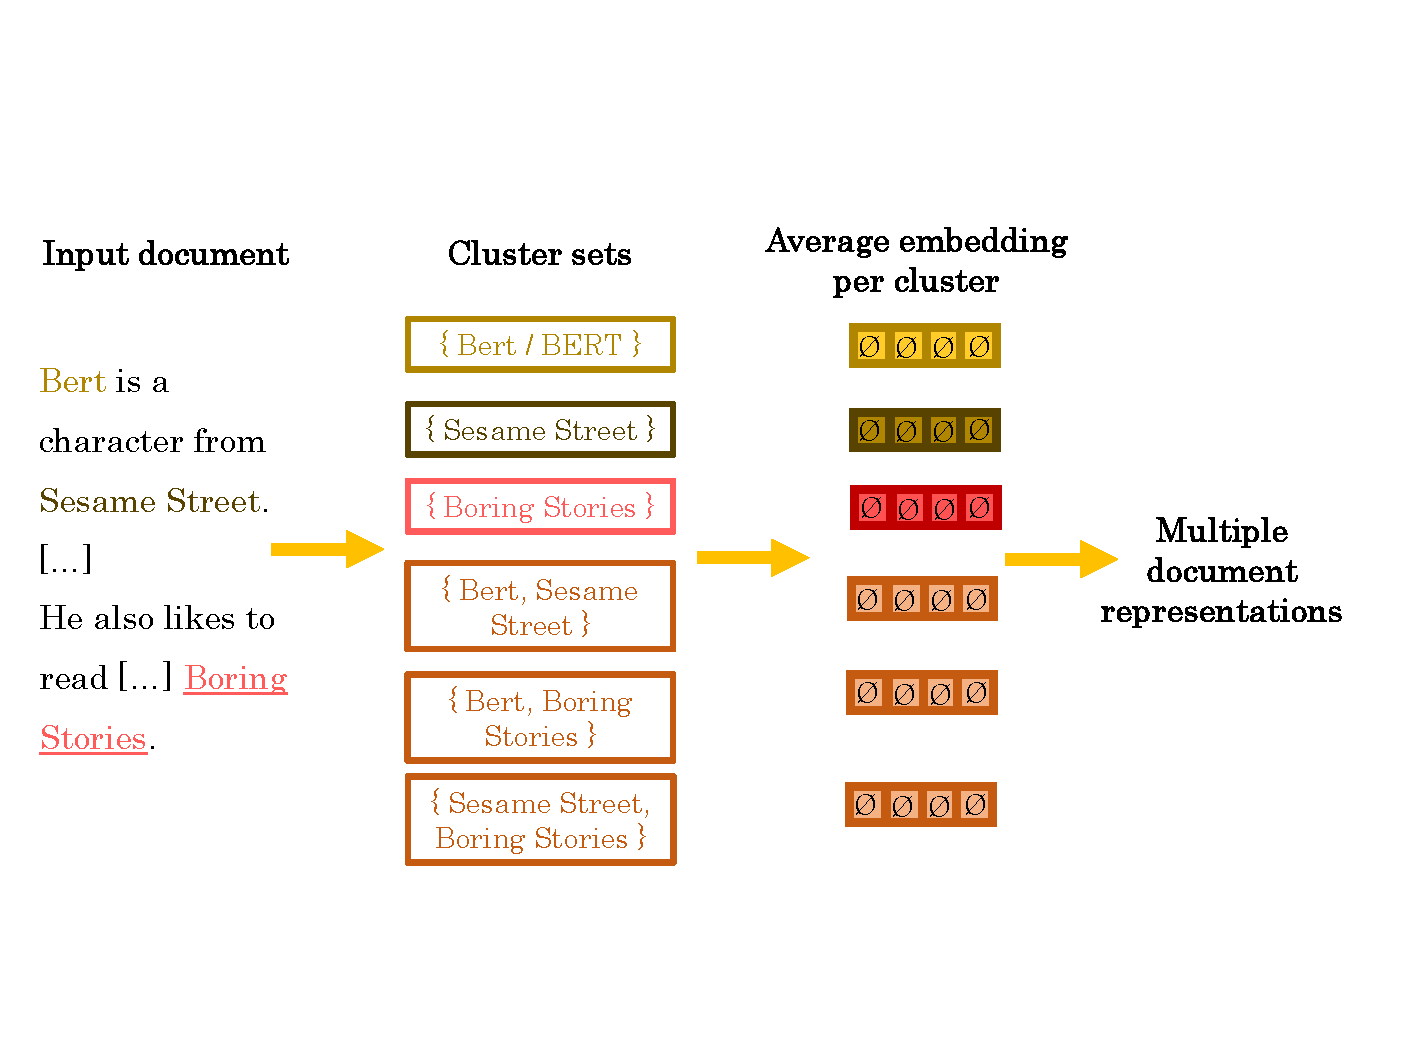
\includegraphics[trim={0cm 3cm 0cm 3.5cm}, clip, width=\textwidth]{resources/eva_multi} 
    \caption{Process of generating entity embeddings for a document following the EVA Multi approach}
    \label{fig:eva_multi}
\end{figure}

All the calculations can be performed independently of the information about queries and thus allow indexing. In contrast to the two previously mentioned methods EVA Single and EVA Single-QA, several entity output embeddings are now generated per document, which have to be taken into account during retrieval ranking. 

\autoref{fig:eva_multi} visualizes the process of generating the embeddings of multiple entity views / clusters. For the given example of three entities within an input document, six different views on entities and document entity representations are generated.



\section{Results}\label{sec:results}

In this section, the concrete implementation of the described models in \autoref{sec:methods} and the resulting results are presented. The focus of the elaborations is on the major findings of the work by Tran and Yates; accordingly, not all results are listed herein. Details can be studied in the paper by Tran and Yates \cite{tran2022dense}.

\subsection{Experimental Setup}

Tran and Yates implemented their models in a TensorFlow (Abadi et al. \cite{abadi2016tensorflow}) setup: For the pretrained language model, they chose a distilled TAS BERT (Sanh et al. \cite{sanh2019distilbert}, Hofstätter et al. \cite{tasbert}), as described in section \ref{subsec:general_model}. To determine the embeddings, they used Dexter (Ceccarelli et al. \cite{ceccarelli2013dexter}) and Wikipedia2Vec (Yamada et. al \cite{yamada2018wikipedia2vec}), as explained in section \ref{subsec:entity_embeddings}. 

Training was conducted using pairwise hinge loss on four Quadro RTX 8000 GPUs in parallel, employing 300,000 training samples from the MS MARCO dataset (Nguyen et al. \cite{nguyen2016ms}). For the models allowing indexing (EVA Single and EVA Multi, see section \ref{subsec:models}), the end-trained model was used to index embeddings for documents. Evaluation was performed on 7,127 test samples from the MS Marco dataset and the datasets TREC Deep Learning (DL) Track 2019 (MacAvaney et al. \cite{trec_dl_2019}), TREC DL 2020 (MacAvaney et al. \cite{trec_dl_2020}), TREC DL HARD (Yates et al. \cite{dl_hard}). Evaluation metrics were chosen to be nDCG@10, MRR@10, MAP@1000.

The models proposed by Tran and Yates (EVA Single, EVA Single-QA, and EVA Multi, as described in section \ref{subsec:models}) were compared against various baselines as BM-25, TAS BERT, ERNIE and others. Details can be examined within the paper by Tran and Yates \cite{tran2022dense}.
\begin{comment}
\begin{itemize}
    \item BM25: The most prominent example of exact matching paradigm, using sparse representations (Robertson et al. \cite{BM25})
    \item TAS BERT: Fine-tuned BERT model using topic-aware sampling strategy as described in \autoref{subsec:general_model}.
    \item ANCE: A state-of-the-art bi-encoder model that employs a sophisticated negative sample mining strategy during training process (Xiong et al. \cite{xiong2020approximate}).
    \item BM25 + T5 (Zero-Shot): First stage ranking using BM25 plus a T5-cross-encoder (Nogueira et al. \cite{nogueira2020document}) to rerank the top 1000 results of first stage retrieval.
    \item ERNIE: Fine-tuned model of ERNIE v2 (Sunh et. al. \cite{sun2020ernie}), which is an optimized version of base ERNIE as described in \autoref{sec:related_work}.
    \item ERNIE Multi: Similar to the EVA Multi approach, but using ERNIE as a pre-trained language model for word embeddings.
    \item Best Reported: The best results of the MS MARCO leader board or respectively the best results of the corresponding papers of the TREC DL datasets (MacAvaney et al. \cite{trec_dl_2019}, MacAvaney et al. \cite{trec_dl_2020}, Yates et al. \cite{dl_hard}).
\end{itemize}
\end{comment}

\subsection{Efficiency}\label{sec:efficiency}

In terms of efficiency, particular attention is paid to latency, and the results for all models under examination are presented in \autoref{tab:results_effectiveness}. The table displays the average search time per query across evaluation datasets for each model, executed on the same server.

\def\arraystretch{1.2}
\begin{table}[!htb]
    \scriptsize
    \centering
    \begin{tabular}{l|l}
    \textbf{Methods}                                        & \textbf{Latency (ms)} \\ \hline
    \textit{\textbf{Low latency (\textless{}100 ms)}}       & \textit{\textbf{}}    \\ \hline
    BM25                                                    & 13                    \\
    ANCE                                                    & 25                    \\
    ERNIE Tuned                                             & 29                    \\
    ERNIE Multi                                             & 70                    \\
    TAS BERT                                                & 28                    \\
    EVA Single                                              & 40                    \\
    EVA Multi                                               & 76                    \\
    EVA Multi-KNRM                                          & 74                    \\ \hline
    \textit{\textbf{Higher latency (\textgreater{}100 ms)}} & \textit{\textbf{}}    \\ \hline
    EVA Single-QA                                           & 2,039                  \\
    EVA Single-QA-KNRM                                      & 3,839                  \\
    BM25 + T5 (Zero-Shot)                                   & 5,052                  \\ \hline
    Best Reported                                           & -                    
    \end{tabular}
    \caption{Analysis of effectiveness of EVA models and baselines}
    \label{tab:results_effectiveness}
\end{table}

\subsection{Effectiveness}\label{sec:effectiveness}

The effectiveness results of the various models applying nDCG@10, MRR@10, MAP@1000 consistently hold across all combinations of evaluation metrics and datasets. To avoid redundancy, this report will provide exemplary results based on the nDCG@10 metric and the TREC DL Track 2019 dataset \cite{trec_dl_2019}. These exemplary results are illustrated in a visual format in \autoref{fig:results}. Further details on the main outcomes can be found in the subsequent section \ref{subsec:outcomes}.

\begin{figure}[!htb]
    \centering
    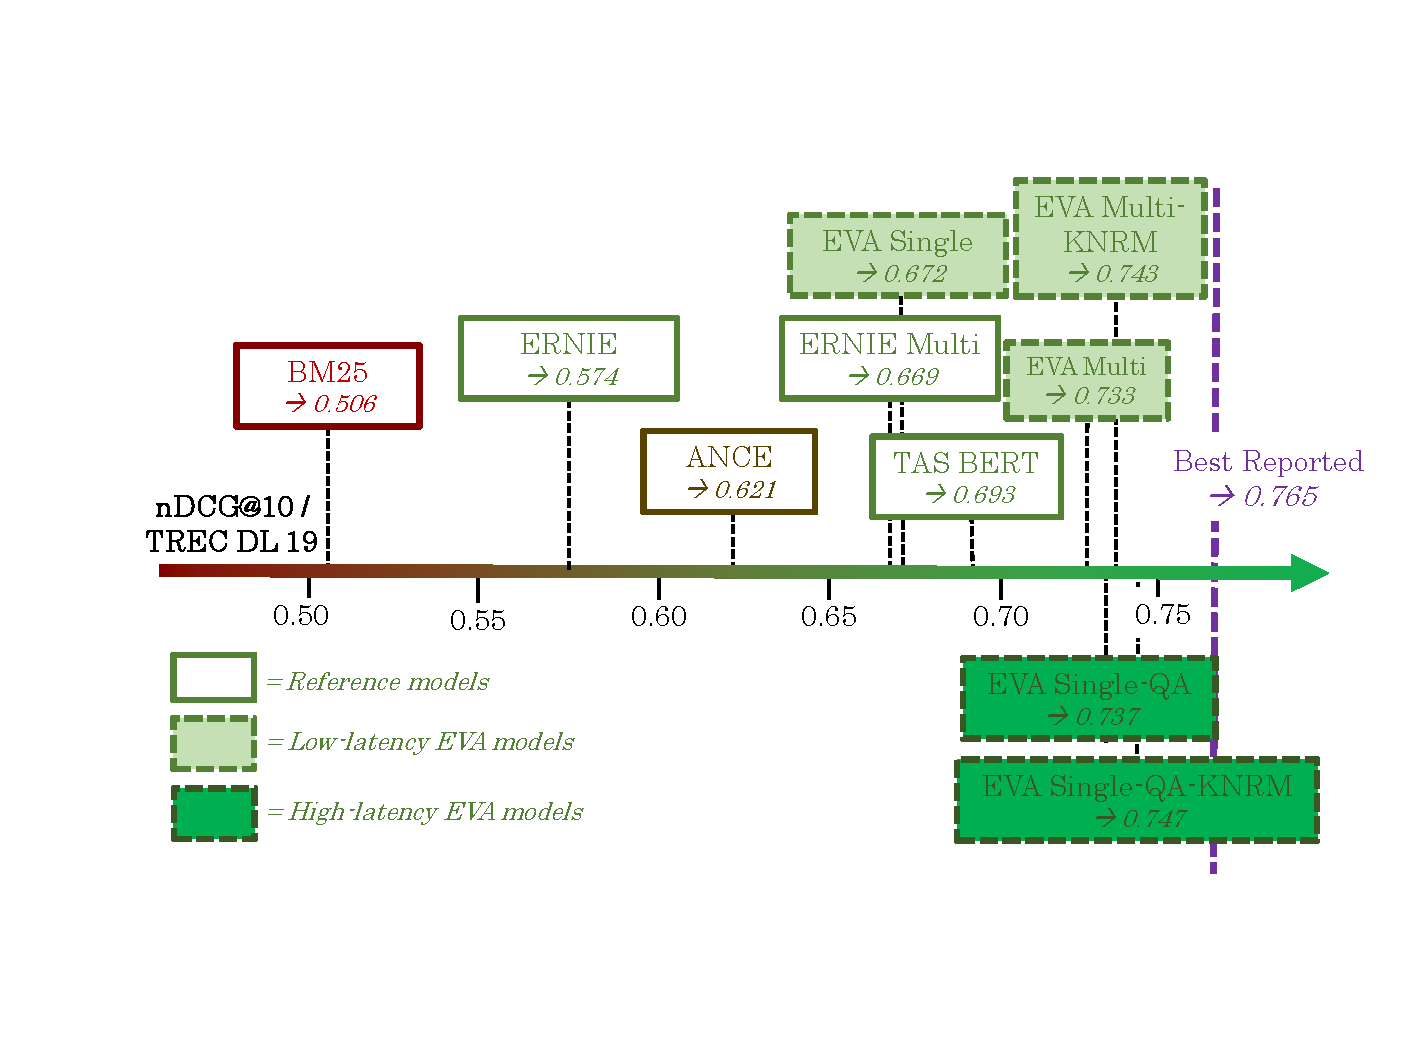
\includegraphics[trim={1.5cm 3cm 0.7cm 3cm}, clip, width=0.85\textwidth]{resources/results} 
    \caption{Exemplary results of EVA models and baselines for TREC DL 19 dataset and evaluation metric nDCG@10}
    \label{fig:results}
\end{figure}

\subsection{Impact}\label{subsec:outcomes}

The outcomes of Tran and Yates' work, based on the results from section \ref{sec:effectiveness} and section \ref{sec:efficiency}, is summarized as follows:

\textbf{Enriching pre-trained language models with entity embeddings improve effectiveness significantly}:
The effectiveness results demonstrate that the models proposed by Tran and Yates, namely EVA Multi and EVA Single-QA, both with and without KNRM signal, outperform the various baselines. In the example presented in \autoref{fig:results}, the nDCG@10 value for the best performing baseline, TAS BERT, is 0.693. In contrast, the values for EVA Multi and EVA Single-QA are 0.733 and 0.737. Moreover, the models only marginally deviate from the best reported results. For MS Marco dataset this refers to MS Marco leaderboard, for the other datasets to the reported benchmarks in the corresponding paper (MacAvaney et al. \cite{trec_dl_2019}, MacAvaney et al. \cite{trec_dl_2020}, Yates et al. \cite{dl_hard}).

\textbf{Multiple entity views increase performance to single view}:
The initial approach, EVA Single, which incorporates entities in documents without a specific focus on the query information, exhibits poor results and even underperforms the baseline TAS BERT. This is due to the inclusion of entirely irrelevant entities within documents during the retrieval process, leading to biased results (see section \ref{subsec:models}). However, when considering only entities relevant to the respective query, as in the cases of EVA Single-QA and EVA Multi, a significant increase in effectiveness is observed compared to all baselines, as explained earlier.

\textbf{KNRM signal provides slight improvement of effectiveness}:
The comparison of the results for the EVA models with and without the additional KNRM signal shows slightly better performance for the models with the KNRM signal. This is evident in the exemplary results of \autoref{fig:results}, where the EVA Multi KNRM model achieves an nDCG@10 value of 0.748, slightly higher than the value of 0.733 for the EVA Multi model. A similar observation is made for the EVA Single-QA model. However, the effect is modest, as the EVA Multi approach outperforms the same approach with the additional KNRM signal in the case of the TREC DL 2020 dataset. In conclusion, the impact of introducing entity embeddings is more significant than that of introducing the KNRM signal.

\textbf{Removing known query assumptions has minor impact on effectiveness, but increases efficiency drastically}:
EVA Multi and EVA Single-QA demonstrate the most effective outcomes, as evidenced in \autoref{fig:results}. The crucial distinction between these models lies in the assumption of knowing queries at runtime for EVA Single-QA and the need for pre-trained language model inference at runtime (see section \ref{subsec:models}). This leads to substantial differences in latency compared to the EVA Multi model. As shown in \autoref{tab:results_effectiveness}, the query latency for the EVA Multi models is 74 ms with KNRM signal and 76 ms without, whereas the latency for both EVA Single-QA models exceeds two seconds. In real-world scenarios, such prolonged latency times are impractical, as users typically expect faster results. However, given that the effectiveness results of EVA Multi and EVA Single-QA only differ marginally, the EVA Multi approach provides a good compromise between efficiency and effectiveness.

\section{Discussion \& Criticism}\label{sec:discussion}

Tran and Yates propose an approach that demonstrates the significant improvement of classical dense retrieval methods through the incorporation of entity information. The results, surpassing the baselines TAS BERT and ERNIE, support the effectiveness of their method. Several positive aspects and some limitations of their work can be identified.

\subsection{Positives}

\begin{itemize}
\item Satisfying results: As demonstrated in \autoref{subsec:outcomes}, Tran and Yates' approach outperforms the baselines, justifying the introduction of their method.
\item Simple and intuitive approach: The ideas and explanations provided by Tran and Yates are straightforward to follow. The introduced methods, from the general model (see \autoref{subsec:general_model}) to the algorithms used (e.g., algorithm \ref{alg:query-aware-entity-representation}), have a clear structure. For instance, the choice of aggregation method for embeddings of word tokens and entities, i.e. concatenation of embeddings (see \autoref{fig:general_model}), is easier to understand than alternative approaches like max pooling or sum pooling. Based on that, the system could be extended with additional embeddings without much effort.
\item Consideration of both effectiveness and efficiency: While many research efforts focus solely on achieving top results on leader boards, Tran and Yates' approach appears to be more oriented towards practical use and sustainability. The EVA Multi-approach offers both high effectiveness and efficiency.
\end{itemize}

\subsection{Negatives}

\begin{itemize}
\item Entities aren't universally relevant: Tran and Yates concentrate solely on the impact of entities in their work, but their analyses reveal that for many queries, entities play no significant role. As shown in \autoref{tab:query_statistics}, 43.5 \% of all queries in the training data do not contain entities, causing the EVA models being ineffective for such queries.
\item Lack of originality: The ideas presented by Tran and Yates are based on existing frameworks, and their contribution mainly lies in the composition of ideas from other authors. As a result, the approach, while intuitive, cannot be classified as groundbreaking. This is evident from the limited citations of their work so far, with only one citation in Kamphuis et al. \cite{kamphuis2023mmead}.
\end{itemize}

\subsection{Possible Extensions}
The granular structure of Tran and Yates' models allows for possible extensions through the exchange or addition of individual components. For instance, the pre-trained language model used to calculate word-level embeddings could be extended beyond the two baseline models TAS BERT and ERNIE to other, more sophisticated models. In domain-specific use cases, a tailored choice of the pre-trained model might further enhance effectiveness. For example, in a biomedical context, BioBERT (Lee et. al \cite{lee2020biobert}) could be considered.

The embedding component for entities could also be replaced or supplemented with other choices. For example, keyword embeddings, as presented by Gab{'\i}n et al. \cite{gabin2023keyword}, or structural information, such as that presented by Raman et al. \cite{raman2022structure}, could serve as alternative sources for external embeddings. Furthermore, in the context of HTML files, Guo et al.'s approach \cite{guo2022webformer} could be explored for generating embeddings.

These extensions could address some limitations of the current approach and potentially lead to further improvements in effectiveness and applicability in different domains.







% References (Literaturverzeichnis):
% a) add ``Literatur'' to table of content
\newpage
\addcontentsline{toc}{section}{References}
% b) Style (with abbreviations: use alpha):
\bibliographystyle{plainnat}
% c) The File:
\bibliography{report}

\end{document}
